\documentclass{llncs}

\usepackage[english]{babel}
%\usepackage[tight]{subfigure}
%\usepackage{floatrow}
\usepackage{graphicx}
%\usepackage{amsmath}
%\usepackage{multirow}
%\renewcommand*\arraystretch{1.25} % extra vertical space in cells
\usepackage{amsmath}
\usepackage[latin1]{inputenc} % pour les caracteres francais dans les remarques

\usepackage[usenames]{color}
\newcommand{\SC}[1]{{\color{red}{\textbf{SC: #1}}}}
\newcommand{\OC}[1]{{\color{blue}{\textbf{OC: #1}}}}
\newcommand{\CD}[1]{{\color{magenta}{\textbf{CD: #1}}}}

%\newcommand{\SC}[1]{}
%\newcommand{\OC}[1]{}
%\newcommand{\CD}[1]{}

\newcommand{\nomore}[1]{}

\begin{document}


\title{Shell Model for Reconstruction and Real-Time Simulation of Thin Anatomical Structures}
%\author{Olivier Comas, St\'ephane Cotin and Christian Duriez}
%\institute{INRIA, Alcove team, Lille, France}

\maketitle

\begin{abstract}
This paper presents a new modelling technique for the deformation of thin anatomical structures like membranes and hollow organs. We show that the behaviour of this type of tissue can be abstracted with a modelling of their surface elastic resistance using shell theory. In order to apply the shell theory in the particular context of medical simulation, our method propose to base the geometrical reconstruction of the organ on the shape functions of the shell element. Moreover, we also use these continuous shape functions to handle the contacts and the interactions with other types of deformable tissues. The technique is illustrated using several examples including the simulation of an angioplasty procedure.
\end{abstract}

\section{Introduction}

The human body is composed of various deformable anatomical structures. Realistic modelling of organ deformations is a challenging research field that opens the door to new clinical applications including: medical training and rehearsal systems, patient-specific planning of surgical procedure and per-operative guidance based on simulation. In all these cases the clinician needs fast update of the deformation model to obtain a real-time display of the computed deformations. To develop this kind of interactive systems, one faces the trade-off problem between accuracy of the model and the need for fast computations. 
Another key challenge of soft-tissue modelling is the variousness of the mechanical behaviours. It seems unrealistic to target a unique model for all tissues even if there are obvious advantages to make maximum use of optimised generic models. Yet most of previous work focus on volumetric models that are able to capture the behaviour of solid organs like the liver or the brain (see for instance \cite{Miller07} \cite{Delingette08}). In contrast, this paper seeks to propose a solution for simulating, in real-time, the deformation of thin anatomical structures whose volume is negligible compared to their surface area. Examples of such anatomical structures include hollow structures, such as the wall of blood vessels, or membranes,  such the capsule of Glisson.

Shell theory allows the modelling of structure deformations when the thickness is small compared to its other dimensions~\cite{Liu03}. The key idea is to model the physical shell as a surface but endowed with mechanical properties in the form of elastic resistance to stretching and bending forces. 
Rather than resorting to shell theory, previous work on medical simulation often relies on linear or angular mass-spring models as in \cite{Nedel98,Hammer08}. Yet, such models are limited in their ability to describe certain behaviour, as they do not rely on continuum mechanics: it is difficult to derive spring stiffness (in particular for angular springs) from elastic properties (Young's modulus and Poisson's ratio).
The use of fast shell based model for computer graphics and interactive simulation was recently introduced with the work of Choi et al.~\cite{Choi07}. The model relies on simplified energy functions and precomputed modal analysis. It allows for fast and visually realistic results. We propose to rely on a similar approach but with more accuracy in order to be applicable to medical simulation. Our model is not based on modal analysis but uses a co-rotational formulation and polynomial shape functions presented in~\cite{Comas2010ISBMS}. 

In this paper, we propose for the first time to apply this technique for modelling the deformations of some anatomical structures. The first step is to geometrically model the surface of the structures using curved triangular shell elements. 
This process is quite similar to the reconstruction of the surface of objects in computer vision. Indeed calculating curvature maps of 3D surfaces represented as digitized data (point clouds or triangulated meshes) has been extensively studied. One of the most common approach is to use continuous surface patches~\cite{Kolb95,Douros02}. The surface is locally approximated by an analytic representation called surface patch, usually chosen to be an implicit surface.
These works target non noise-sensitive approaches and coherent surface and curve extraction from 3D data~\cite{Tang99}.
%In~\cite{Tang99} an elegant and non noise-sensitive approach that infers sign and direction of principal curvatures directly from the input is presented and the authors use this information for coherent surface and curve extraction from 3D data. 
However, our situation is substantially different as %extracting the surface is not our ultimate goal. 
we want to model the deformation of the structure. 
%In that regard the curvature of the surface has a physical meaning: it represents the rest shape of our anatomical structure, that is the configuration with zero energy. 
%\CD{Non !!! Rien ne te dit que l'objet ne te dit que l'objet n'est pas d�form� au moment o� tu prend l'image !!!}
In that regard the curvature of the surface has a physical meaning: it represents the neutral fiber surface of the shell modelling on which the plane stress hypothesis~\cite{Liu03} applies. 
Therefore we propose to match the shape (polynomial) functions used in our shell FEM formulation to describe the surface of the shells with the surface of the anatomical structures that we wish to simulate.


One originality of this work is that the polynomial shape functions, defined on  curved triangles, are used in three different ways to optimize the computation and reach real-time computations.
The shell model, presented in section~\ref{sec:model}, uses them to computes the internal forces using a Finite Element Modelling (FEM).
The interactions with other models, including deformable solid models, are captured and processed using the same polynomial interpolations.
Moreover, in section~\ref{sec:mesh} we also present an automatic process to obtain meshes from image based reconstruction that relies on the exact same polynomial functions.
% in an attempt to optimise the computation using fewer elements. 
Finally the benefits of our approach (meshing of a curved surface, fast computation and possible interactions with solid models) are illustrated using various examples presented in section~\ref{sec:results}.

\section{Co-rotational triangular shell model for thin structures}
\label{sec:model}

A complete description and validation of our co-rotational triangular shell finite element model is available in one of our previous publication \cite{Comas2010ISBMS}. Therefore we will only remind briefly the key points. We improved and extended a plate model first introduced by Przemieniecki \cite{Przemieniecki68} to a co-rotational formulation. Co-rotational approaches offer a good trade-off between computational efficiency and accuracy by allowing small deformations but large displacements. Once combined with an in-plane membrane formulation we obtain an accurate, yet computationally efficient, shell finite element method featuring both membrane and bending energies. 
In the following, we detail the bending stiffness computation in order to present the polynomial shape functions that are used in the shell model.


%\paragraph{Triangular elastic membrane}

%The element stiffness matrix $\textbf{K}_e$ can be computed as follows:

%\begin{equation}
%\textbf{K}_e = \int_v \textbf{J} \boldsymbol{\chi} \textbf{J}^{T} dV
%\end{equation}
%where $\textbf{J}$ is the strain-displacement matrix and $\boldsymbol\chi$ embodies the material's behaviour. The stiffness matrix in the global frame is eventually obtained using the rotation matrix of the element: $\textbf{K} = \textbf{R}^{T} \textbf{K}_e \textbf{R} $ where $\textbf{R}$ describes the rotation of the (triangular) element with respect to its initial configuration.

\paragraph{Polynomial shape function}
%
\begin{figure}
\vspace{-1.0cm}
\centering
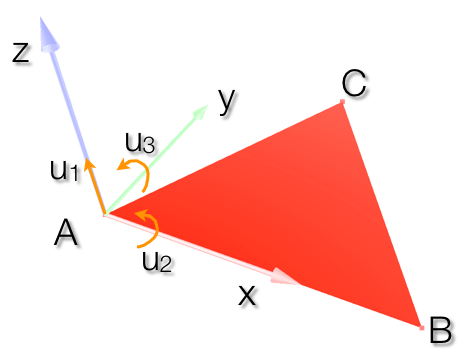
\includegraphics[height=4cm]{images/bending}
\caption {The different degrees of freedom $u$ of a triangular thin plate in bending.}
\label{fig-triangle}
\vspace{-0.5cm}
\end{figure}
%
To calculate the stiffness matrix for the transverse deflections and rotations shown on figure \ref{fig-triangle}, the deflection $u_z$ is computed using a polynomial interpolation:
\begin{equation}
 u_z = c_1 + c_2x + c_3y + c_4x^2 + c_5xy + c_6y^2 + c_7x^3 + c_8xy^2 + c_9y^3
\label{eq-deflection}
\end{equation} 
where $c_1$, \ldots , $c_9$ are constants. Using a third-degree polynomial expression allows us to reach a greater precision for both the computation of the bending energy and the interpolation within the surface of the shell. Let us define the vector $\textbf{u} = \left\{u_1 u_2 \ldots u_9 \right\} $ of the displacements and slopes at the three corners of the triangular plate using the following notations:
\begin{equation}
u_1 = (u_z)_{x_1,y_1} \hspace{1cm} u_2 = \left(\frac{\partial u_z}{\partial y}\right)_{x_1,y_1} \hspace{1cm} u_3 = - \left(\frac{\partial u_z}{\partial x}\right)_{x_1,y_1}
\end{equation} 
and so on for the two other vertices.
We then can derive a matrix $\textbf{C}$ such as $\textbf{u} = \textbf{Cc}$ where $\textbf{c} = \left\{c_1 c_2 \ldots c_9 \right\} $.
We can calculate the strains from the flat-plate theory using:
\begin{equation}
\label{eq-deformation}
e_{xx} = -z \frac{\partial^2u_z}{\partial x^2}
\hspace{1cm}
e_{yy} = -z \frac{\partial^2u_z}{\partial y^2}
\hspace{1cm}
e_{xy} = -2z \frac{\partial^2u_z}{\partial x \partial y}
\end{equation} 


Symbolically this may be expressed as $\textbf{e} = \textbf{Dc}$ where $\textbf{D}$ derives from equations~\ref{eq-deflection} and~\ref{eq-deformation}. Noting that $\textbf{c} = \textbf{C}^{-1}\textbf{u}$, we have $\textbf{e} = \textbf{DC}^{-1}\textbf{u} = \textbf{bu}$ where the strain-displacement matrix $\textbf{b} = \textbf{DC}^{-1}$. 
The stiffness matrix $\textbf{K}_e$ for an element is then obtained from:
\begin{equation}
\textbf{K}_e = \int_v \textbf{b}^{T} \boldsymbol\chi \textbf{b} dV
\end{equation} 
where $\boldsymbol\chi$ is the material matrix. The stiffness matrix in the global frame is eventually obtained using the rotation matrix of the element. %as in the membrane case. 

\paragraph{Mechanical interactions with the curved surface of shells}
\label{sec:interactions}
The practical interest of modelling complex behaviours such as bending and twisting would remain fairly low for medical simulation if contacts and constraints were not handled properly. In our case the difficulty comes from different sources. First the collision detection must be carried out with the curved surface of shell elements as opposed to the classic detection on plane triangles. Then forces applied to a given triangle need to be distributed between linear forces and torques onto its three vertices.  As we will see, the same polynomial interpolation function (\ref{eq-deflection}) chosen to compute the bending energy in our FEM formulation is also used to capture the interactions between the curved surface and other objects. 

In order to detect the collision with the bent surface, we have chosen the subdivision approach. Therefore a finer mesh is created by adding vertices on the surface of each element. We first sample the flat surface of each element by recursively dividing each triangle into four smaller ones and the deflection of each new vertex is computed using (\ref{eq-deflection}) and the displacements and slopes at the three vertices of the triangular element. This process of subdivision allows us to render each shell as a curved triangle (Fig.~\ref{fig-shell} (a) and (b)) and detect any collision with the curved surface of the shell using any of the classic collision detection algorithms working on flat triangles.
\begin{figure}
\centering
\vspace{-0.5cm}
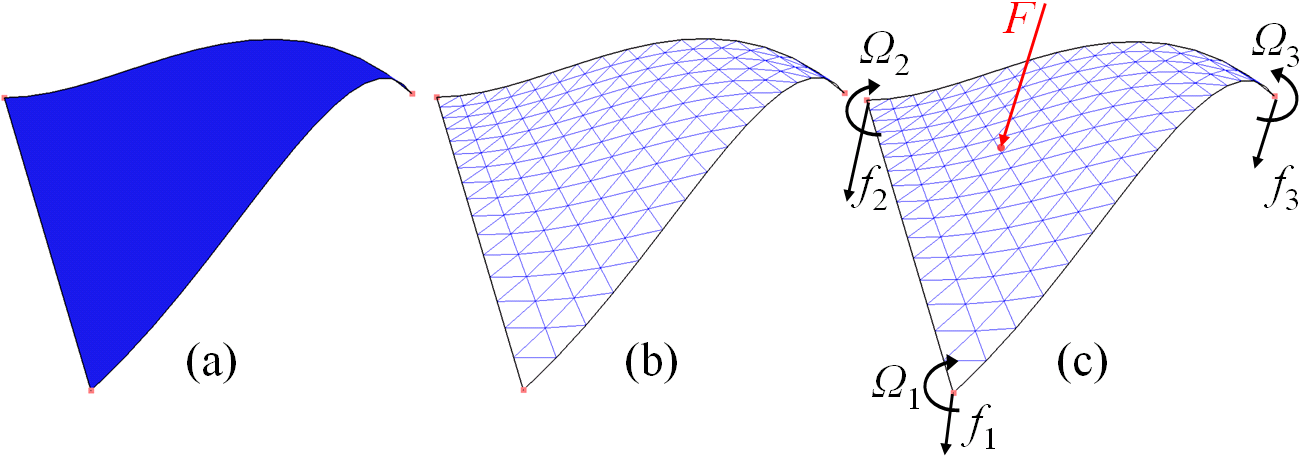
\includegraphics[height=3.5cm]{images/shell_curvature2.png}
\vspace{-0.3cm}
\caption {(a)  The triangle formed by the three vertices of the shell has been recursively subdivided 3 times and the deflection of each new vertex was computed according to the same deflection function used in our shell finite element formulation. (b) Sampling the actual surface of the shell allows rendering and more accurate collision detection. (c) The shape function is used to distribute an external force $F$ on the triangle nodes}

\label{fig-shell}
\vspace{-0.4cm}
\end{figure}

Once a collision has been detected, it must be processed by distributing the linear force received on the bent surface between the three vertices of the triangle. First the linear part of the force is simply transmitted on each node using the barycentric coordinates of the contact point's projection onto the triangle. 

The main difficulty is to convert the normal component of the force applied to the bent surface into a torque at each of the three nodes (Fig.~\ref{fig-shell} (c)). Our approach is the following: during force computation, we use the angle measured at each node to compute the local deflection of each subvertex within the triangle. Differentiating the formulation twice yields a relation between the torque applied at each node and the generated force in bending. We therefore need to invert the latter formulation to convert a bending force into torques at each vertex. We start by retrieving the normal component of the applied force vector $F_{\mathrm{z}}$. We project the application point of the force into the triangle's plane and compute its local coordinates $(x,y)$. We create the polynom $P = F_{\mathrm{z}}(1 \hspace{0.2cm} x \hspace{0.2cm} y \hspace{0.2cm} x^2 \hspace{0.2cm} xy \hspace{0.2cm} y^2 \hspace{0.2cm} x^3 \hspace{0.2cm} xy^2 \hspace{0.2cm} y^3)^T$. The moments at each vertex are then obtained with $\Omega = (\textbf{C}^{-1})^T P$.  Thus we are able to transmit any force coming from elaborate interactions with the curved surface of shells to the mechanical vertices used in our FEM formulation. 

\section{A mechanically-driven method to mesh curved surfaces with shells}
\label{sec:mesh}
%\paragraph{Related work}

%Another key component of finite element methods is the mesh of the simulated object being used. While a sufficient number of elements is needed to accurately describe the geometry, too many of them will yield a computationally expensive simulation and solving the system in real-time may no longer be possible. Literature about volumic mesh generation algorithms is fairly dense. However, there are only a few that are concerned about the generation of meshes over curved surfaces. One of the most widely used techniques for the creation of surface meshes is the plane to surface transformation method \cite{Zienkiewicz71}, mesh is first generated on a two-dimensional domain and then mapped onto the surface. If this method gives reasonably good meshes on smooth surfaces, the results are usually quite poor with more complex curved surfaces. The finite elements may be generated directly on the curved surfaces based on the advancing front technique \cite{Lo85,Lau96}. The main issue with this approach is that an analytical description of the geometry is needed, which is not the case in medical simulation. Another method consists of using an a priori error estimator to build an adaptive mesh generation \cite{Baumann97}. However, the tolerance of this indicator should be chosen depending on the desired accuracy of the finite element solution, and therefore requires some knowledge about the problem in order to choose an effective tolerance. In \cite{Bechet02} the authors start from an existing triangular mesh created with a CAD software and refine and smooth the mesh based on element quality and surface curvature. While all those methods allow their authors to get satisfactory meshes over curved surfaces according to their needs, they all make use of flat elements to mesh geometries and do not generate actual shells. 

Because the surface of an anatomical structure has a physical meaning, %we cannot use any type of function to reconstruct this surface. The surface must be patched 
we propose to patch the surface with triangular elements whose interpolation makes use of the same shape function designed for our shell FEM formulation. By suggesting a method to reconstruct the surface of any structures with curved shell, the meshing process is optimised. Indeed while many flat triangles are often required to describe highly curved surfaces, fewer triangular shell elements are needed to describe the given geometry with the same precision since they can be naturally curved. In the following we assume that we have a high resolution triangular mesh obtained from a binary segmented image of the organ we want to simulate (via a Marching Cube algorithm for instance). Our goal is to create a mesh featuring the optimal number of shell elements while staying as close as possible to our targeted geometry. 

Therefore we need to insure that the distance between the surface of our shell-based mesh and the targeted high resolution mesh will be minimal. An efficient technique for measuring the error between two surfaces is the Hausdorff distance \cite{Klein96,Cignoni98}. As a reminder the Hausdorff distance between two meshes is the maximum between the two so-called one-sided Hausdorff distances:
\begin{equation}
d_{\mathrm{H}}(X,Y) = \max \left\{ \sup_{x \in X} \inf_{y \in Y} d(x,y), \sup_{y \in Y} \inf_{x \in X} d(x,y) \right\} \enspace .
\end{equation}
where $d()$ is the Euclidian distance between two points. The same technique of subdivision used for rendering allows us to sample the actual surface described by the shells to compute the Hausdorff distance with the targeted high resolution mesh. 

The first step in the process of generating a shell-based mesh is an aggressive simplification of the targeted high resolution mesh by using the quadric edge collapse decimation technique implemented in Meshlab \cite{Meshlab}. The algorithm tries as much as possible to preserve mesh boundaries and generate high quality triangular elements. We then apply a heuristic method derived from the work of Saupin et. al \cite{Saupin07} with tetrahedral meshes based on very simple geometrical rules. For each node of the coarse mesh, we find the three closest triangles on the high resolution mesh and we move the node to the barycenter of the three centres of mass of those triangles. This technique locally smooths the surface of the mesh while converging towards the desired high resolution mesh. At each iteration of this algorithm we measure the error between the curved surface of shells and the target using the Hausdorff distance and the process is stopped when the required precision has been reached. A simple example is shown Fig.~\ref{fig-cylinder} to illustrate the method. 
%We can notice that differences with the target mesh have been subtantially reduced.
% Christian: je ne comprend pas cette phrase.. du coup, je l'enl�ve !

\begin{figure}
\centering
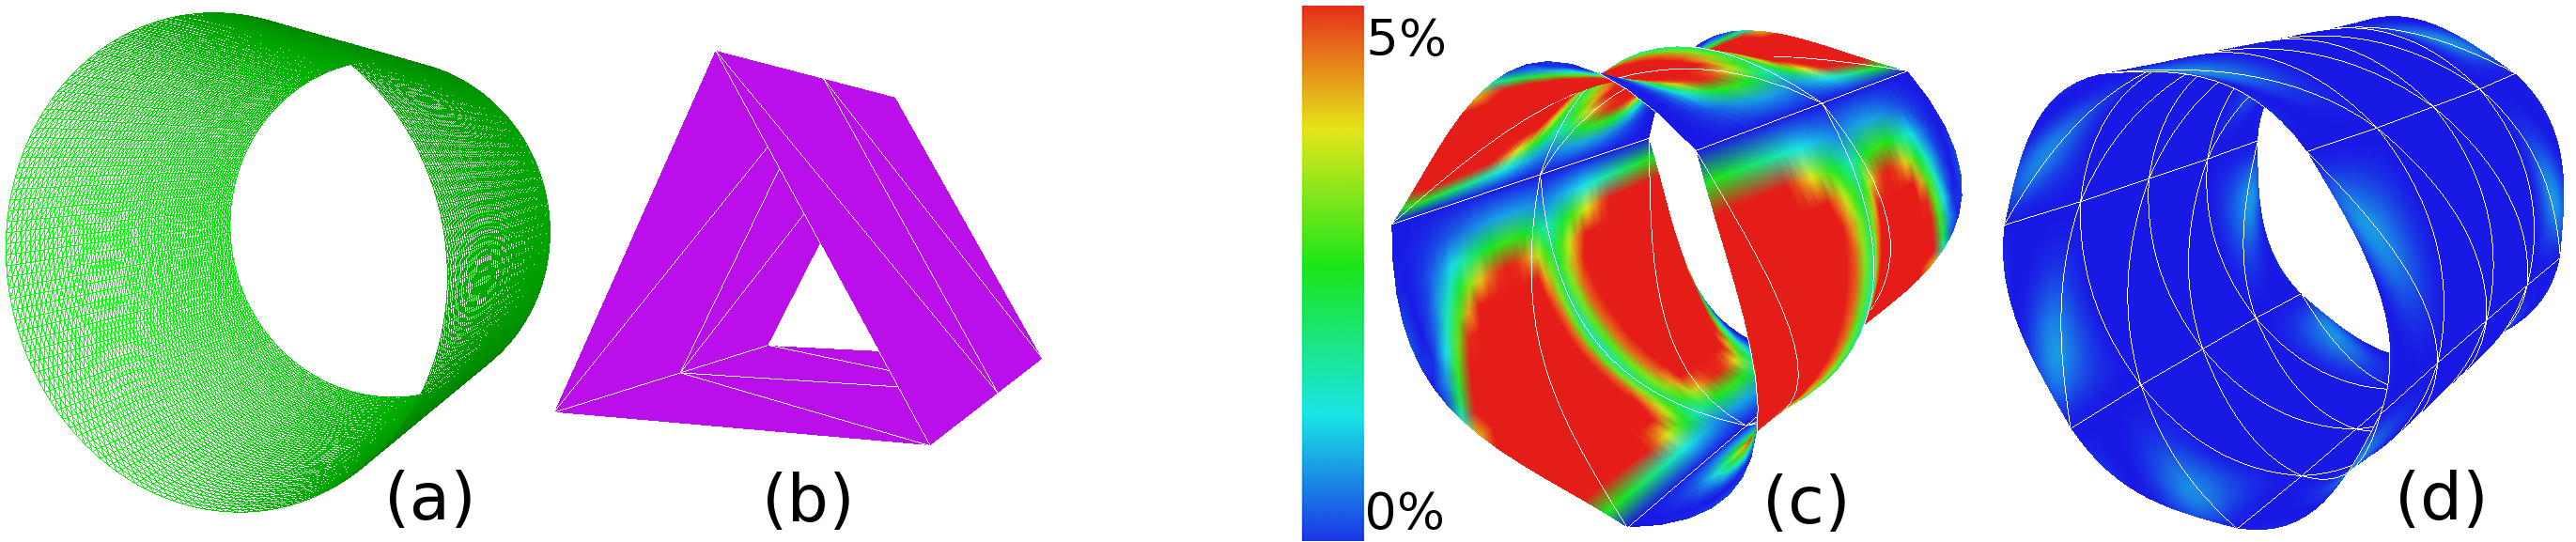
\includegraphics[height=2.5cm]{images/exampleCylinder}
\caption {Illustration of our method on a simple example. The target is a high resolution cylinder mesh of 16,384 triangles (a) and we start from a very coarse mesh (12 triangles) approximating the shape of a cylinder, rendered with flat triangles here (b). In (c) the same coarse mesh is rendered with shells and a one-sided Hausdorff distance colour map is applied to show the initial error with the high resolution mesh. (d) One-sided Hausdorff distance colour map after only one iteration of our algorithm (48 shells).}
\label{fig-cylinder}
\end{figure}

\section{Results}
\label{sec:results}
\paragraph{Meshing of anatomical structures}

This approach has been applied to mesh more complex anatomical structures with curved shell elements. In each case the error is expressed as a percentage of the diagonal of the object's bounding box. 

\begin{figure}
\centering
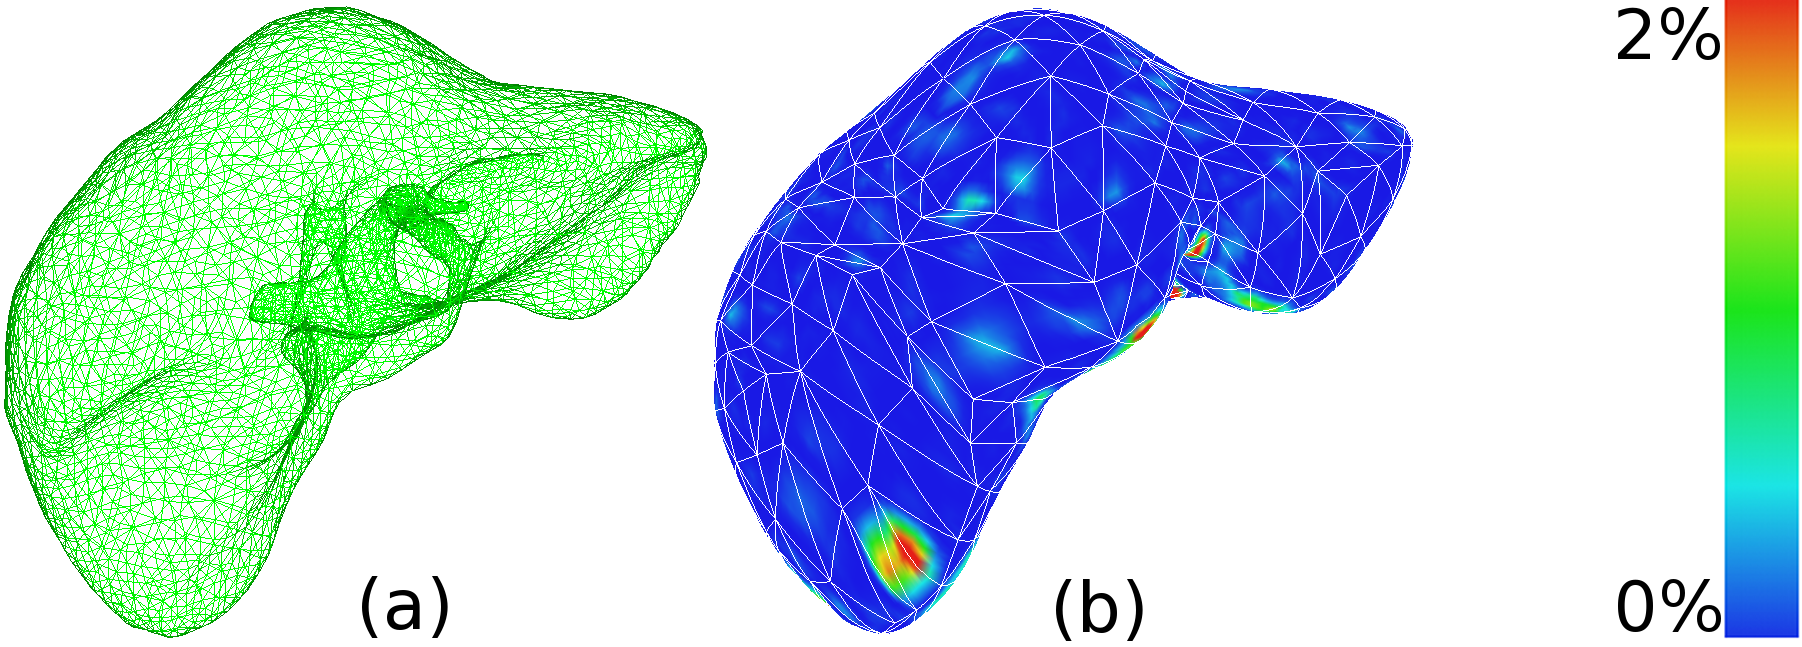
\includegraphics[height=3cm]{images/resultsLiver}
\caption {Left: the targeteted high resolution Glisson's capsule mesh (8,000 triangles). Right: the one-sided Hausdorff distance error map after applying only one iteration of our algorithm to the coarse mesh (1,200 shells)}. 
\label{fig-liver}
\end{figure}

\begin{figure}
\centering
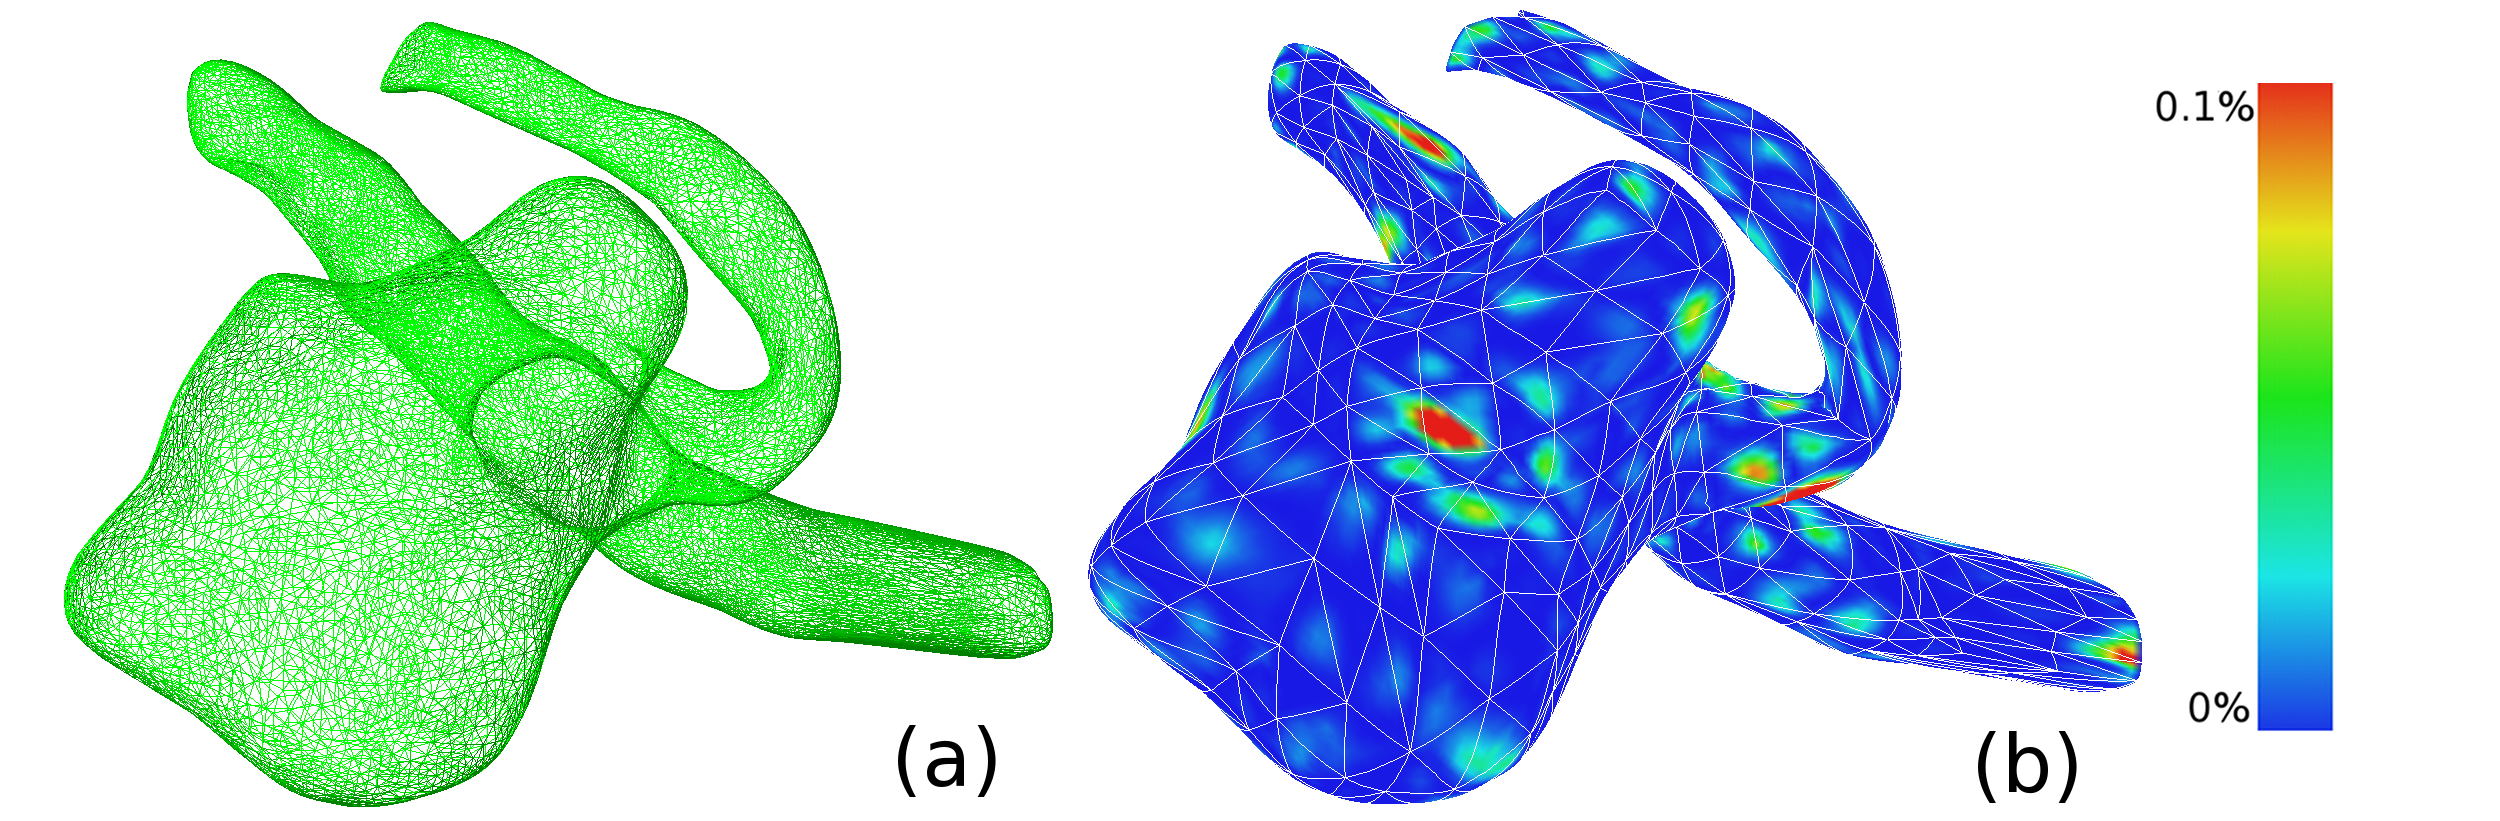
\includegraphics[height=3cm]{images/resultsAneurysm}
\caption {(a) the targeteted high resolution aneurysm mesh (28,368 triangles). (b): the one-sided Hausdorff distance error map on a mesh of 1,160 shells generated with our method \CD{Montre plutot celui qui part de 200 et fait environ 800 triangles a la fin !!!}}.
\label{fig-aneurysm}
\end{figure}


\paragraph{Computation times}

We perform several tests on the aneurysm model at different resolution. 
The shells are resisting to a uniform pressure load and are solved using an Conjugate Gradient (CG) iterative solver.
The computation times are reported in the Fig.\ref{fig-computation}. 
Implicit integration allows for large time steps (40ms) and the computation is real-time for 800 shell elements and a reasonable error criterion ($5\%$).
When the computation time must be bounded (critical real-time applications), one can fix the number of CG iterations to, for instance, $100$ and remain real-time for 1000 shell elements. However, in that case, the accuracy of the results are not checked.

\begin{figure}
\centering
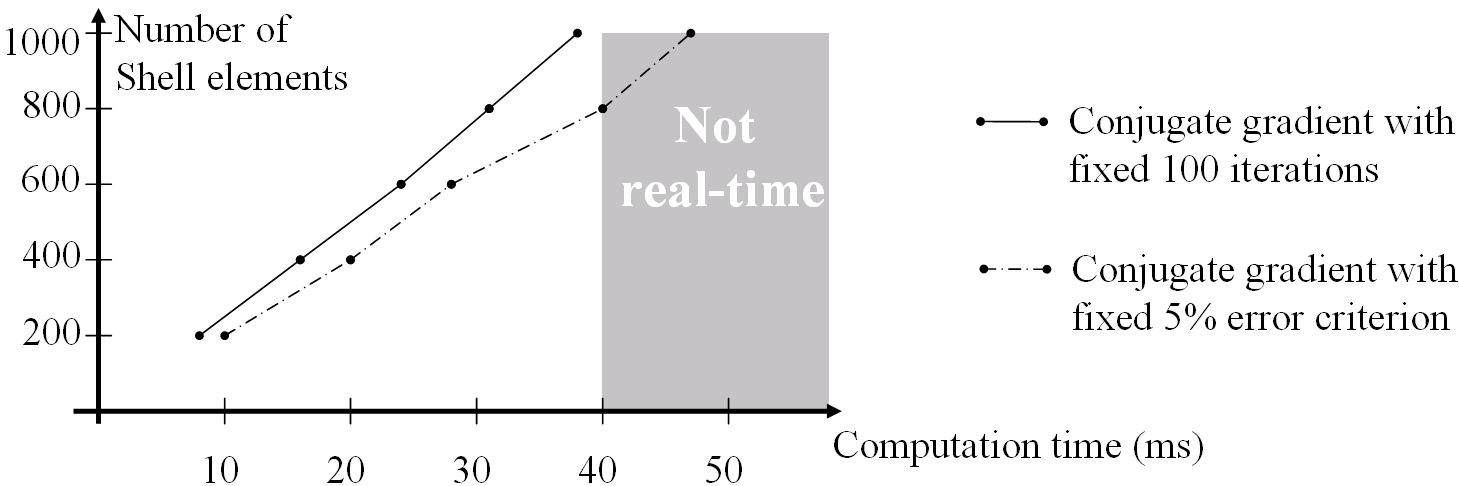
\includegraphics[height=3cm]{images/computation_time.png}
\caption {Computation time on meshes of the Aneurysm model with 200, 400, 600, 800 and 1000 elements.}.
\label{fig-computation}
\end{figure}

\paragraph{Coupling between tetrahedra and shells for advanced modelling}

Structures in human body can be either solid (brain, liver, prostrate etc.) or hollow (blood vessels, colon, stomach etc.). However knowing how to model the two kind of structures is not sufficient to reach a high degree of accuracy in medical simulation. Indeed real life situations are more complex. As an example, the external surface of the liver is covered by a single layer of cells called Glisson's capsule. Its interaction with the liver plays an important role into the overall structure's mechanical behaviour. Therefore considering the interaction between solid and hollow objects is as crucial as modelling the two structures separately. 

An example of medical procedure to illustrate this point even further is angioplasty. Angioplasty is the technique of mechanically widening a narrowed or obstructed blood vessel, typically as a result of atherosclerosis. An empty and collapsed balloon on a guide wire, known as a balloon catheter, is passed into the narrowed locations and then inflated to a fixed size using water pressures. The balloon crushes the fatty deposits, so opening up the blood vessel to improved flow. As a proof of concept we tried to simulate an angioplasty (Fig.~\ref{fig-stent}). The blood vessel is modelled using the shell FEM formulation described in this paper and the fatty deposits are simulated with a tetrahedral FEM method and are fixed to the interior wall of the blood vessel. When the balloon inflates it crushes the deposits and the deposits then apply a pressure onto the curved surfaces of shells modelling the interior wall. The forces are then distributed onto the mechanical nodes of the blood vessel mesh as detailled in section \ref{sec:interactions}, which widens the blood vessel as expected. 

\begin{figure}
\centering
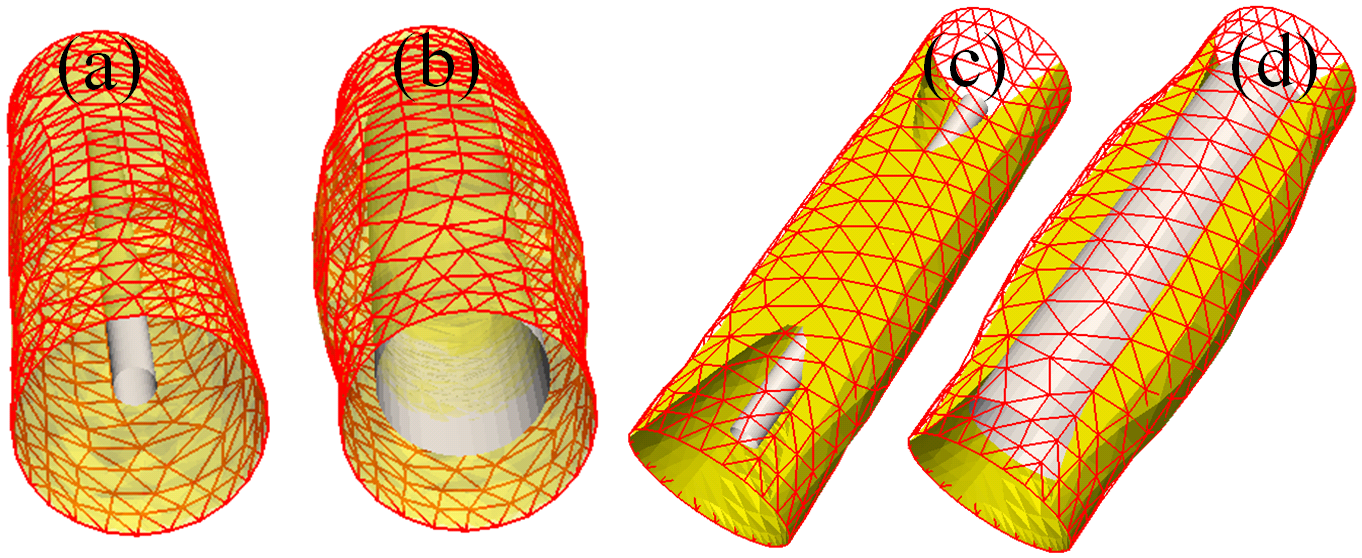
\includegraphics[height=3.8cm]{images/stenose_final.png}
\caption {Simulation of an angioplasty procedure. (a) The collapsed balloon was inserted into the blood vessel simulated with our shell FEM formulation. The fatty deposits (in yellow) are modelled with a tetrahedral FEM. (b) Upon inflation the balloon is crushing the fatty deposits, which is applying a pressure onto the interior wall and widening the blood vessel.}
\label{fig-stent}
\end{figure}


\section{Conclusion}
We proposed a complete framework for real-time modelling of thin anatomical structures. The novelty of our method relies on the combination of a shell finite element formulation and a geometric surface reconstruction both based on the same polynomial interpolation function used to describe the surface of shells. We also showed how contacts and interactions with the curved surfaces of shells could be handled using the same function. The efficiency of the whole approach was demonstrated through shell reconstruction and real-time modelling of a blood vessel showing signs of an aneurysm. Finally these results are very encouraging towards fine modelling of more complex situations like interactions existing between the liver and the Glisson's capsule or the simulation of an angioplasty procedure. 

%\section*{Acknowledgments}

\bibliographystyle{splncs}
\bibliography{bibliography}

\end{document}
